% !TEX root = ../multi_task.tex

In this section, we present the experimental results we did not include in the main text. %We give tabulated multi-label classification errors in Section~\ref{sec:multi_label_error} and present an additional ablation study in Section~\ref{sec:additional_ablation}.

%\subsection{Multi-label classification results}
\label{sec:multi_label_error}
In the main text, we plotted a radar chart of the binary attribute classification errors. However, we did not include the tabulated results due to the space limitations. Here we list the binary classification error of each attribute for each algorithm in Table~\ref{tab:multi_label_table}.


\begin{table}[ht]
\caption{Multi-label classification error per attribute for all algorithms.}
\newcolumntype{Z}{S[table-format=2.2,table-auto-round]}
\resizebox{\textwidth}{!}{%
\begin{tabular}{l@{\hspace{2mm}}ZZ@{\hspace{2mm}}ZZ@{\hspace{2mm}}Z@{}c@{\hspace{10mm}}l@{\hspace{2mm}}ZZ@{\hspace{2mm}}ZZ@{\hspace{2mm}}Z}
\toprule
 & \multicolumn{1}{c}{Uniform}  &  \multicolumn{1}{c}{Single}  &  \multicolumn{1}{c}{Kendall } &      \multicolumn{1}{c}{Grad} &              &         &        &  \multicolumn{1}{c}{Uniform}  &  \multicolumn{1}{c}{Single}  &  \multicolumn{1}{c}{Kendall}  &  \multicolumn{1}{c}{Grad}& \\
   &  \multicolumn{1}{c}{scaling}  &   \multicolumn{1}{c}{task}    &   \multicolumn{1}{c}{et al.}    &   \multicolumn{1}{c}{Norm}            &  \multicolumn{1}{c}{Ours} &   &  & \multicolumn{1}{c}{scaling} &   \multicolumn{1}{c}{task} &   \multicolumn{1}{c}{et al.}   &   \multicolumn{1}{c}{Norm}   & \multicolumn{1}{c}{Ours} \\
\midrule \\
Attr. 0 & 7.11 & 7.16 & 7.18 & 6.54 & \bftabnum 6.17 & & Attr. 5 & 4.91 & 4.75 & 4.95 & 4.19 & \bftabnum 4.13 \\
Attr. 1 & 17.30 & \bftabnum 14.38 & 16.77 &  14.80 & 14.87 & & Attr. 6 & 20.97 & 14.24 & 15.17 & \bftabnum 14.07 &  14.08 \\
Attr. 2 & 20.99 & 19.25 & 20.56 & 18.97 & \bftabnum 18.35 & & Attr. 7 & 18.53 & 17.74 & 18.84 & 17.33 & \bftabnum 17.25 \\
Attr. 3 & 17.82 & 16.79 & 18.45 & 16.47 & \bftabnum 16.06 & & Attr. 8 & 10.22 & 8.87 & 10.19 & 8.67 & \bftabnum 8.42 \\
Attr. 4 & 1.25 & 1.20 & 1.17 & 1.13 & \bftabnum 1.08 & & Attr. 9 & 5.29 & 5.09 & 5.44 & 4.68 & \bftabnum 4.60 \\
\midrule
Attr. 10 & 4.14 & 4.02 & 4.33 & 3.77 & \bftabnum 3.60 & & Attr. 15 & 0.81 & \bftabnum 0.52 & 0.62 & 0.56 & 0.56 \\
Attr. 11 & 16.22 & 15.34 & 16.64 & 14.73 & \bftabnum 14.56 & & Attr. 16 & 4.00 & 3.94 & 3.99 & 3.72 & \bftabnum 3.46 \\
Attr. 12 & 8.42 & 7.68 & 8.85 & \bftabnum 7.23 &  7.41 & & Attr. 17 & 2.39 & 2.66 & 2.35 & \bftabnum 2.09 &  2.16 \\
Attr. 13 & 5.17 & 5.15 & 5.26 & 4.75 & \bftabnum 4.52 & & Attr. 18 & 8.79 & 9.01 & 8.84 & 8.00 & \bftabnum 7.83 \\
Attr. 14 & 4.14 & 4.13 & 4.17 & 3.73 & \bftabnum 3.54 & & Attr. 19 & 13.78 & 12.27 & 13.86 & 11.79 & \bftabnum 11.29 \\
\midrule
Attr. 20 & 1.61 & 1.61 & 1.58 & \bftabnum 1.42 &  1.43 & & Attr. 25 & 27.59 & 24.82 & 26.94 & 24.26 & \bftabnum 23.87 \\
Attr. 21 & 7.18 & \bftabnum 6.20 & 7.73 & 6.91 & 6.26 & & Attr. 26 & 3.54 & 3.40 & 3.78 & 3.22 & \bftabnum 3.16 \\
Attr. 22 & 4.38 & 4.14 & 4.08 & 3.88 & \bftabnum 3.81 & & Attr. 27 & 26.74 & 22.74 & 26.21 & 23.12 & \bftabnum 22.45 \\
Attr. 23 & 8.32 & 6.57 & 8.80 & 6.54 & \bftabnum 6.47 & & Attr. 28 & 6.14 & 5.82 & 6.17 & 5.43 & \bftabnum 5.16 \\
Attr. 24 & 5.01 & 5.38 & 5.12 & 4.63 & \bftabnum 4.23 & & Attr. 29 & 5.55 & 5.18 & 5.40 & 5.13 & \bftabnum 4.87 \\
\midrule
Attr. 30 & 3.29 & 3.79 & 3.24 & \bftabnum 2.94 &  3.03 & & Attr. 35 & 1.15 & 1.13 & 1.08 & \bftabnum 0.94 &  1.08 \\
Attr. 31 & 8.05 & 7.18 & 8.40 & 7.21 & \bftabnum 6.92 & & Attr. 36 & 7.91 & 7.56 & 8.06 & 7.47 & \bftabnum 7.18 \\
Attr. 32 & 18.21 & 17.25 & 18.15 & \bftabnum15.93 & \bftabnum 15.93 & & Attr. 37 & 13.27 & 11.90 & 13.47 & 11.61 & \bftabnum 11.19 \\
Attr. 33 & 16.53 & 15.55 & 16.19 & 13.93 & \bftabnum 13.80 & & Attr. 38 & 3.80 & \bftabnum 3.29 & 4.04 & 3.57 & 3.51 \\
Attr. 34 & 11.12 & 9.76 & 11.46 & 10.17 & \bftabnum 9.73 & & Attr. 39 & 13.25 & 13.40 & 13.78 & 12.26 & \bftabnum 11.95 \\
\bottomrule
\end{tabular}}
\label{tab:multi_label_table}
\end{table}





\iffalse
\subsection{How dynamic are the resulting weights?}
\label{sec:additional_ablation}
One way to interpret our method is to consider the $\alpha^t$ computed by our method as task weights that are dynamically computed as the solution of a min-norm problem. In Figure~\ref{fig:mnist_scales}, we plot the weights computed by our method for task-L in the Multi-MNIST experiments. As shown in the figure, the resulting weights fluctuate significantly from batch to batch. This implies that a consistent descent direction requires highly dynamic scaling. Given that the losses and uncertainties are relatively smooth during minibatch training, this behavior explains why heuristics like uncertainty weighting \citep{Kendall2018} struggle to find a consistent descent direction. This further substantiates the case for multi-objective modeling for the multi-task learning problem.

\begin{figure}[H]%{r}{0.5\textwidth}
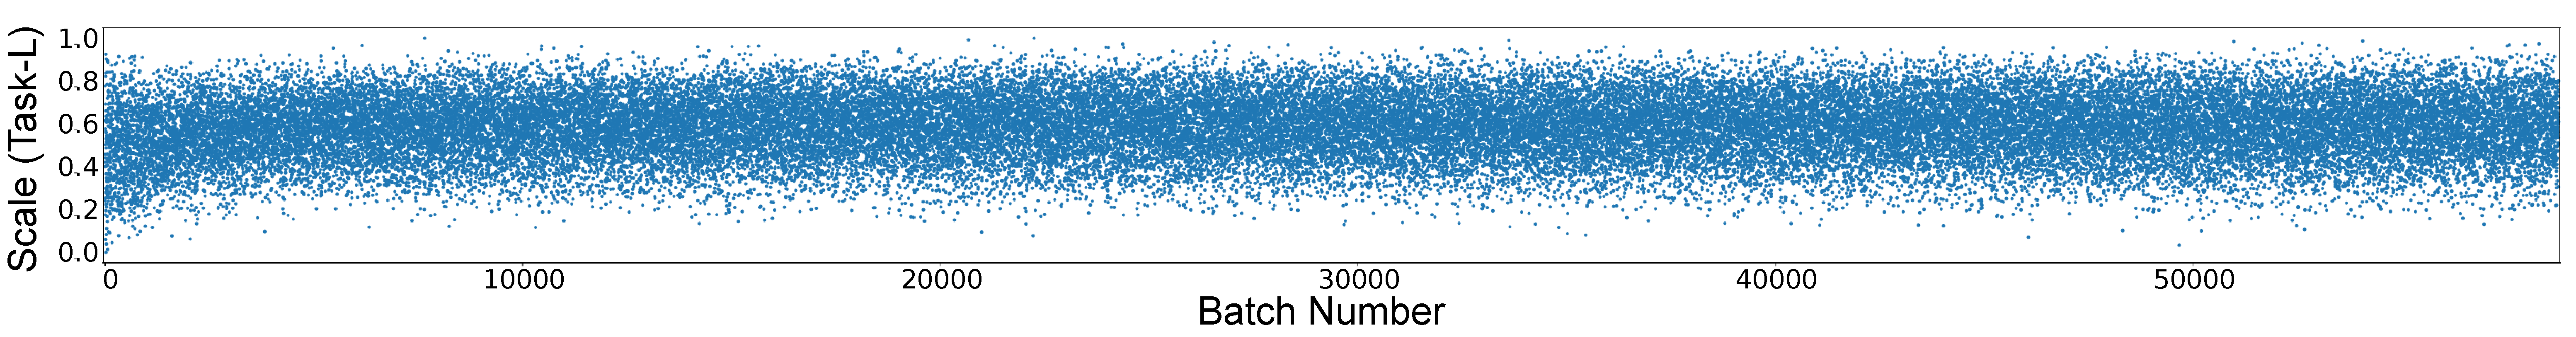
\includegraphics[width=\textwidth]{scale_batch.pdf}
%\vspace{-5mm}
\caption{$\alpha^1$ that our method computes per batch in the MultiMNIST experiment. Although the loss is typically smooth, the required scaling for a consistent descent direction fluctuates significantly.}
\label{fig:mnist_scales}
\end{figure}
\fi